\documentclass[tikz,border=0cm]{standalone}
\usepackage{type1cm}
\usepackage{fp}
\usetikzlibrary{calc}
\usetikzlibrary{shadows}

\usepackage{fetamont}
\usepackage{cmbright}

\usepackage{bm,amsmath,amssymb}
\usepackage{soul}
\usepackage{multirow}

\newcommand{\clm}{Cl\'{e}ment }
\newcommand{\norm}[1]{\lVert#1\rVert}
\newcommand{\semi}[1]{\lvert#1\rvert}

\renewcommand\refname{}   % Don't want references title


\definecolor{edblue}{RGB}{4, 80, 124}
\definecolor{eyellow}{RGB}{248, 176, 23}
\definecolor{elblue}{RGB}{55, 172, 195}

\usepackage[a4paper, margin=1in]{geometry}
\usepackage{url}
\usepackage{setspace}
\renewcommand{\baselinestretch}{1.0}
\let\OLDthebibliography\thebibliography
\renewcommand\thebibliography[1]{
  \OLDthebibliography{#1}
  \setlength{\parskip}{0pt}
  \setlength{\itemsep}{0pt plus 0.3ex}
}

\begin{document}

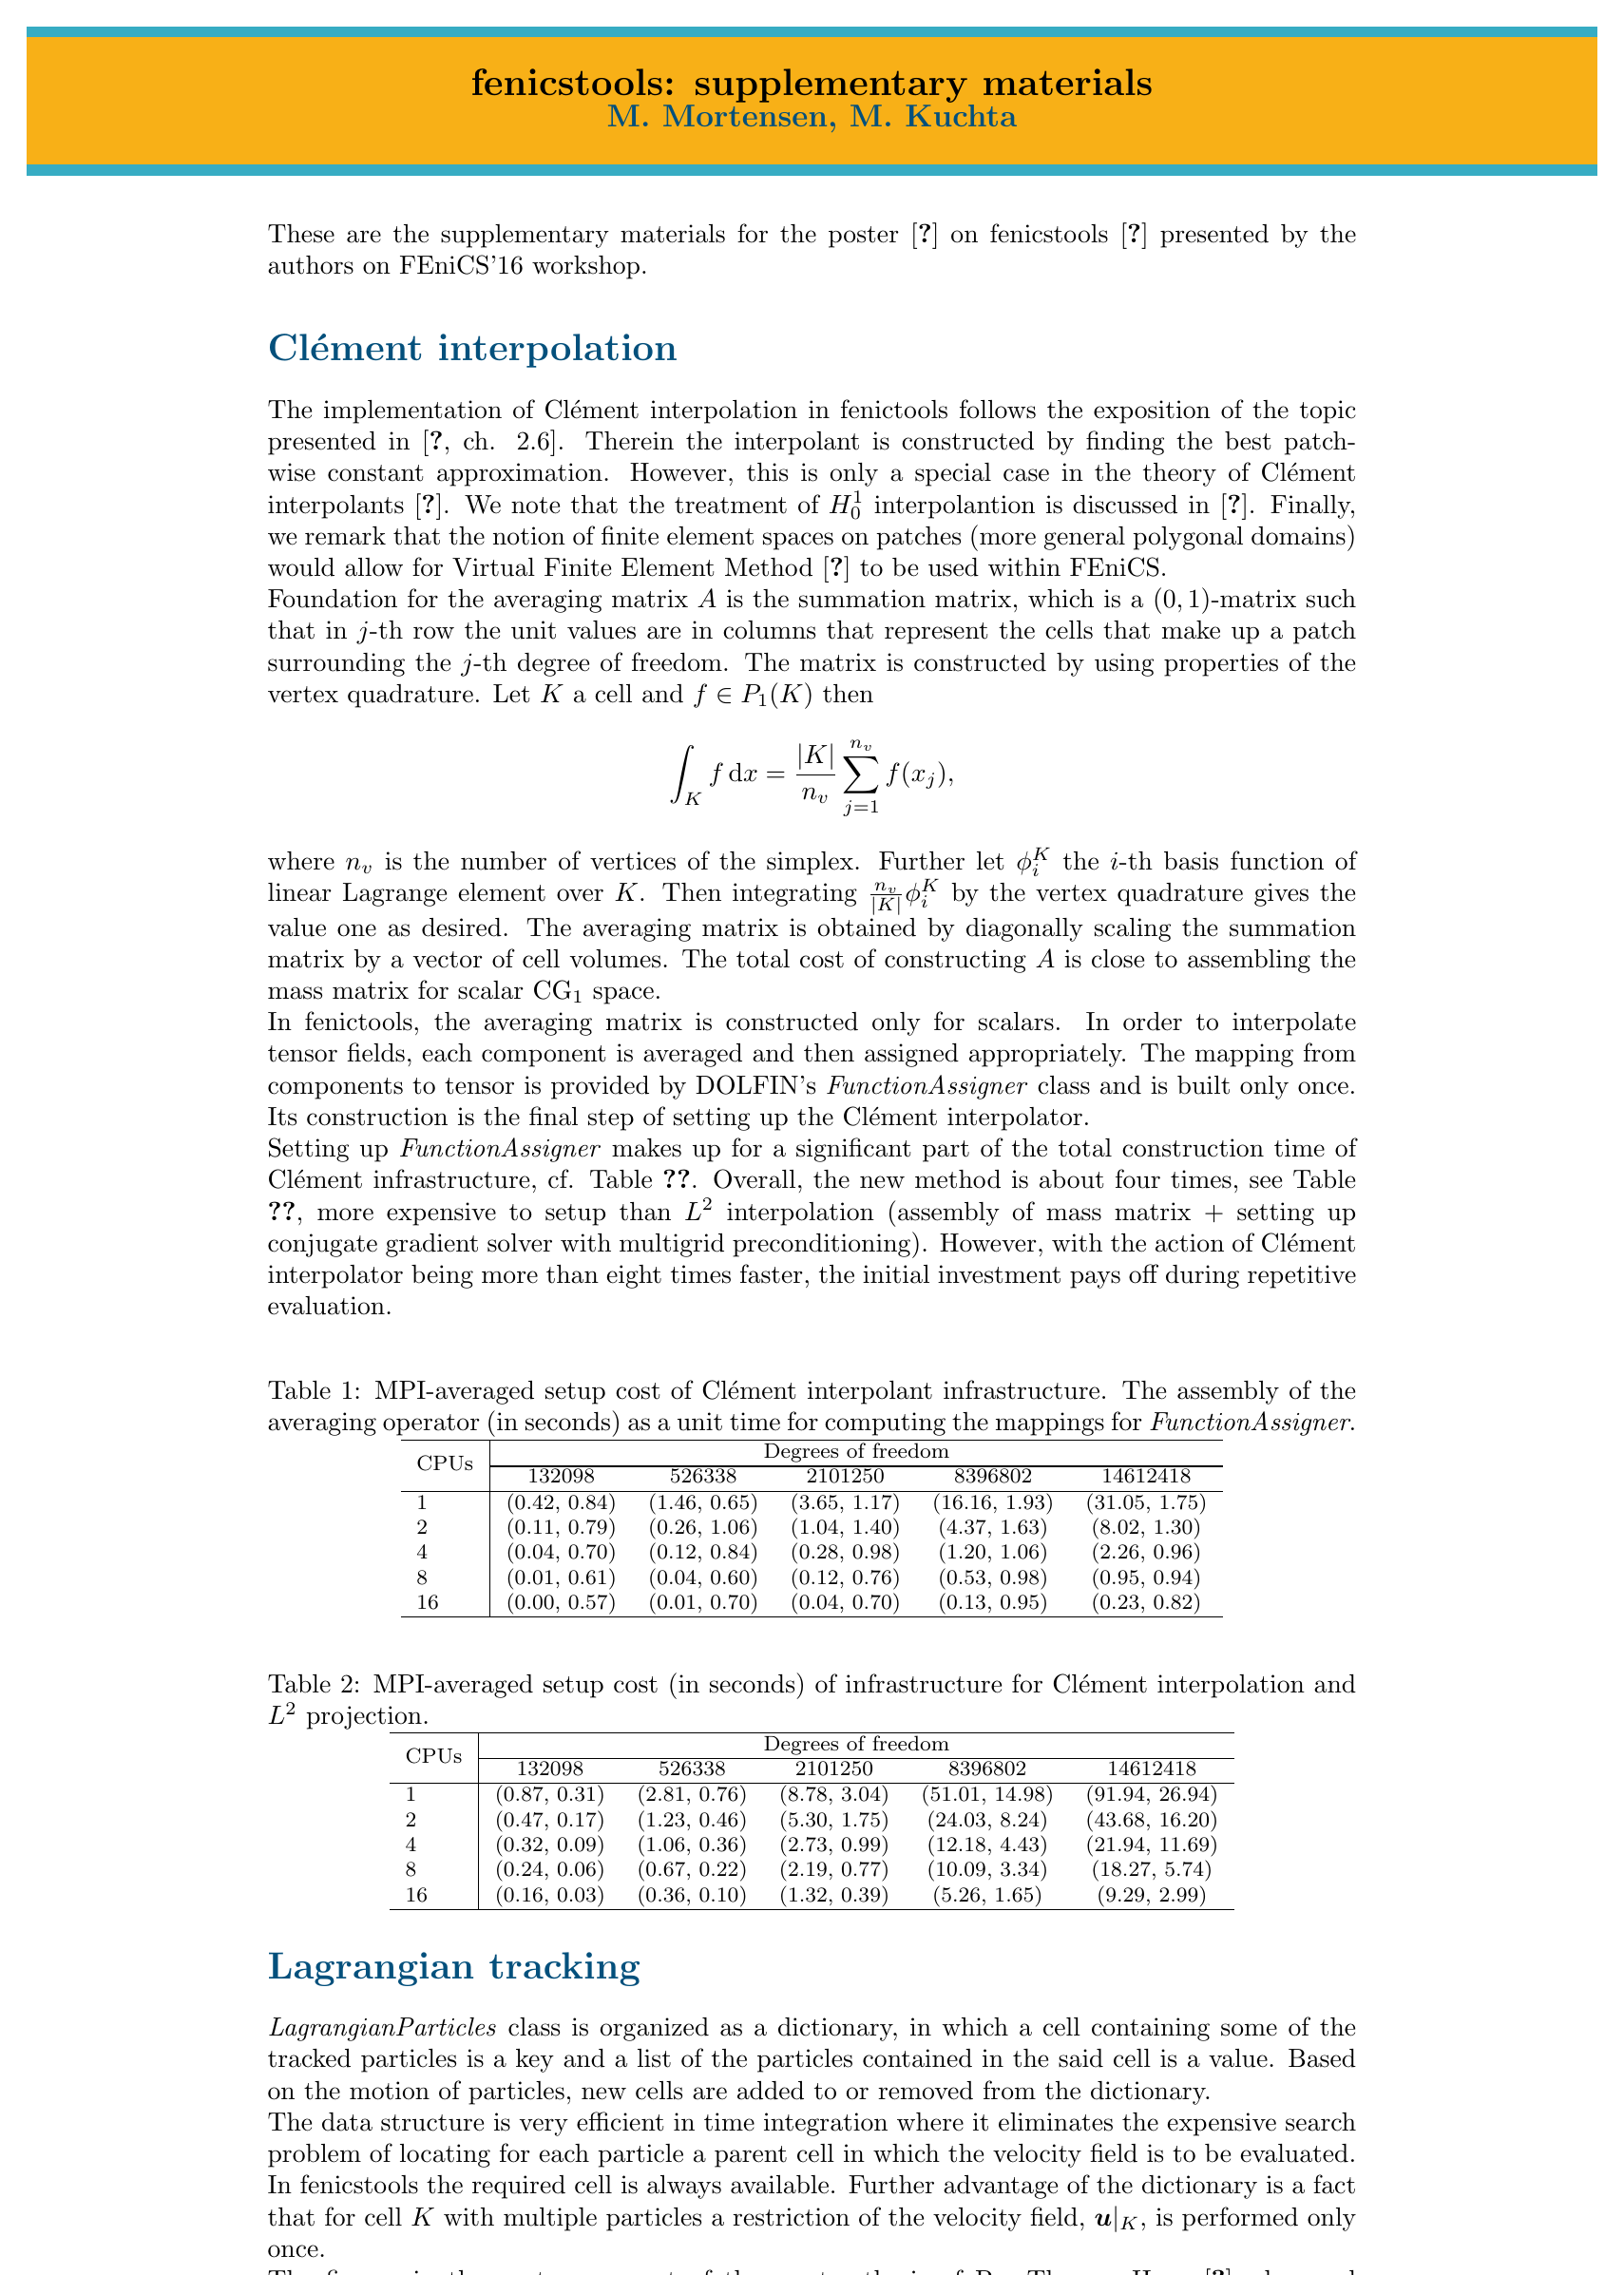
\begin{tikzpicture}[x=21cm, y=29.7cm]
\fill[white, use as bounding box] (0, 0) rectangle (1, 1);

%%%%%%%%%%%%%%%%%%%%%%%%%%
% Title
%%%%%%%%%%%%%%%%%%%%%%%%%%
\begingroup
\draw[fill=eyellow, draw=none] { 
  ($(current bounding box.north west)+(0cm, -20.0mm)$) --
  ($(current bounding box.north east)+(0cm, -20.0mm)$) -- 
  (current bounding box.north east) --
  (current bounding box.north west) -- 
  cycle
};
   %
\draw[elblue, line width=1.5mm]{
  ($(current bounding box.north east)-(0cm, 0.75mm)$) --
  ($(current bounding box.north west)-(0cm, 0.75mm)$)
};
  %
\draw[elblue, line width=1.5mm]{
  ($(current bounding box.north east)+(0cm, -19.25mm)$) --
  ($(current bounding box.north west)+(0cm, -19.25mm)$)
};
\node[anchor=center]
      (title)
      at ($(current bounding box.north)+(0cm, -1.0cm)$)
  {\begin{minipage}{\textwidth}
   \begin{center}
     {\ffmfamily\Large\bfseries\color{black}{fenicstools: supplementary materials}}\\
     {\ffmfamily\large\color{edblue}\textbf{M.~Mortensen, M.~Kuchta}}
   \end{center}
  \end{minipage}};
\endgroup


\node[anchor=north] at ($(current bounding box.north)+(0cm, -2.5cm)$)
{
  \begin{minipage}{1.2\textwidth}
    These are the supplementary materials for the poster \cite{poster} on 
    fenicstools \cite{fenicstools} presented by the authors on FEniCS'16
    workshop.

%%%%%%%%%%%%%%%
% CLM
%%%%%%%%%%%%%%%
    \section*{\ffmfamily\color{edblue}{\clm interpolation}}
    The implementation of \clm interpolation in fenictools follows the
    exposition of the topic presented in \cite[ch. 2.6]{braess}. Therein the
    interpolant is constructed by finding the best patch-wise constant
    approximation. However, this is only a special case in the theory of 
    \clm interpolants \cite{clement}. We note that the treatment of $H^1_0$
    interpolantion is discussed in \cite{scott}. Finally, we remark that the notion
    of finite element spaces on patches (more general polygonal domains) would allow 
    for Virtual Finite Element Method \cite{vfem} to be used within FEniCS.

    Foundation for the averaging matrix $A$ is the summation matrix, which is a 
    $(0, 1)$-matrix such that in $j$-th row the unit values are in columns that 
    represent the cells that make up a patch surrounding the $j$-th degree of
    freedom. The matrix is constructed by using properties of the vertex quadrature. 
    Let $K$ a cell and $f\in P_1(K)$ then
    \[
    \displaystyle \int_{K} f\,\mathrm{d}x = \frac{\semi{K}}{n_v} \sum_{j=1}^{n_v} f(x_j),
    \]
    where $n_v$ is the number of vertices of the simplex. Further let $\phi^K_i$ the
    $i$-th basis function of linear Lagrange element over $K$. Then integrating
    $\tfrac{n_v}{\semi{K}}\phi^K_i$ by the vertex quadrature gives the value one 
    as desired. The averaging matrix is obtained by diagonally scaling the
    summation matrix by a vector of cell volumes. The total cost of constructing
    $A$ is close to assembling the mass matrix for scalar CG$_1$ space.

    In fenictools, the averaging matrix is constructed only for scalars. In
    order to interpolate tensor fields, each component is averaged and then assigned
    appropriately. The mapping from components to tensor is provided by DOLFIN's
    \emph{FunctionAssigner} class and is built only once. Its construction is
    the final step of setting up the \clm interpolator. 
    
    Setting up \emph{FunctionAssigner} makes up for a significant part of the 
    total construction time of \clm infrastructure, cf. Table \ref{tab:assign}. 
    Overall, the new method is about four times, see Table \ref{tab:cstr}, more 
    expensive to setup than $L^2$ interpolation (assembly of mass matrix + setting 
    up conjugate gradient solver with multigrid preconditioning). However, with 
    the action of \clm interpolator being more than eight times faster, the initial 
    investment pays off during repetitive evaluation.

\begin{table}[ht]
\begin{center}
\caption{MPI-averaged setup cost of \clm interpolant infrastructure. The assembly of the
  averaging operator (in seconds) as a unit time for computing the mappings
for \emph{FunctionAssigner}.}
\label{tab:assign}
\footnotesize{
\begin{tabular}{l|ccccc}
\hline
\multirow{2}{*}{CPUs} & \multicolumn{5}{c}{Degrees of freedom}\\
\cline{2-6}
   &     132098 & 526338     &    2101250 &      8396802 & 14612418\\
\hline
  1 & (0.42, 0.84) & (1.46, 0.65) & (3.65, 1.17) & (16.16, 1.93) & (31.05, 1.75)\\
  2 & (0.11, 0.79) & (0.26, 1.06) & (1.04, 1.40) & (4.37, 1.63) & (8.02, 1.30)\\
  4 & (0.04, 0.70) & (0.12, 0.84) & (0.28, 0.98) & (1.20, 1.06) & (2.26, 0.96)\\
  8 & (0.01, 0.61) & (0.04, 0.60) & (0.12, 0.76) & (0.53, 0.98) & (0.95, 0.94)\\
  16 & (0.00, 0.57) & (0.01, 0.70) & (0.04, 0.70) & (0.13, 0.95) & (0.23, 0.82)\\
\hline
\end{tabular}
}
\end{center}
\end{table}
%
\begin{table}
\begin{center}
\caption{MPI-averaged setup cost (in seconds) of infrastructure for \clm interpolation and 
$L^2$ projection.}
\label{tab:cstr}
\footnotesize{
\begin{tabular}{l|ccccc}
\hline
\multirow{2}{*}{CPUs} & \multicolumn{5}{c}{Degrees of freedom}\\
\cline{2-6}
   &     132098 & 526338     &    2101250 &      8396802 & 14612418\\
\hline
  1 &  (0.87, 0.31) & (2.81, 0.76) & (8.78, 3.04) & (51.01, 14.98) & (91.94, 26.94)\\
  2 &  (0.47, 0.17) & (1.23, 0.46) & (5.30, 1.75) & (24.03, 8.24) & (43.68, 16.20)\\
  4 &  (0.32, 0.09) & (1.06, 0.36) & (2.73, 0.99) & (12.18, 4.43) & (21.94, 11.69)\\
  8 &  (0.24, 0.06) & (0.67, 0.22) & (2.19, 0.77) & (10.09, 3.34) & (18.27, 5.74)\\
  16 & (0.16, 0.03) & (0.36, 0.10) & (1.32, 0.39) & (5.26, 1.65) & (9.29, 2.99)\\
\hline
\end{tabular}
}
\end{center}
\end{table}

%%%%%%%%%%%%%%%
% LP
%%%%%%%%%%%%%%%
    \section*{\ffmfamily\color{edblue}{Lagrangian tracking}}
    \emph{LagrangianParticles} class is organized as a dictionary, in which a
    cell containing some of the tracked particles is a key and a list of the
    particles contained in the said cell is a value. Based on the motion of
    particles, new cells are added to or removed from the dictionary. 
    
    The data structure is very efficient in time integration where it eliminates 
    the expensive search problem of locating for each particle a parent cell in 
    which the velocity field is to be evaluated. In fenicstools the required
    cell is always available. Further advantage of the dictionary is a fact that
    for cell $K$ with multiple particles a restriction of the velocity field, 
    $\boldsymbol{u}|_K$, is performed only once.

    The figures in the poster are part of the master thesis of Per Thomas Haga
    \cite{ptthesis} who used \emph{LagrangianParticles} to study drug delivery
    in spinal chord. The thesis developed into a recently submitted paper 
    \cite{ptpaper}.

  \end{minipage}
};
\end{tikzpicture}

%%%%%%%%%%%%%%%%
% Refences
%%%%%%%%%%%%%%%%
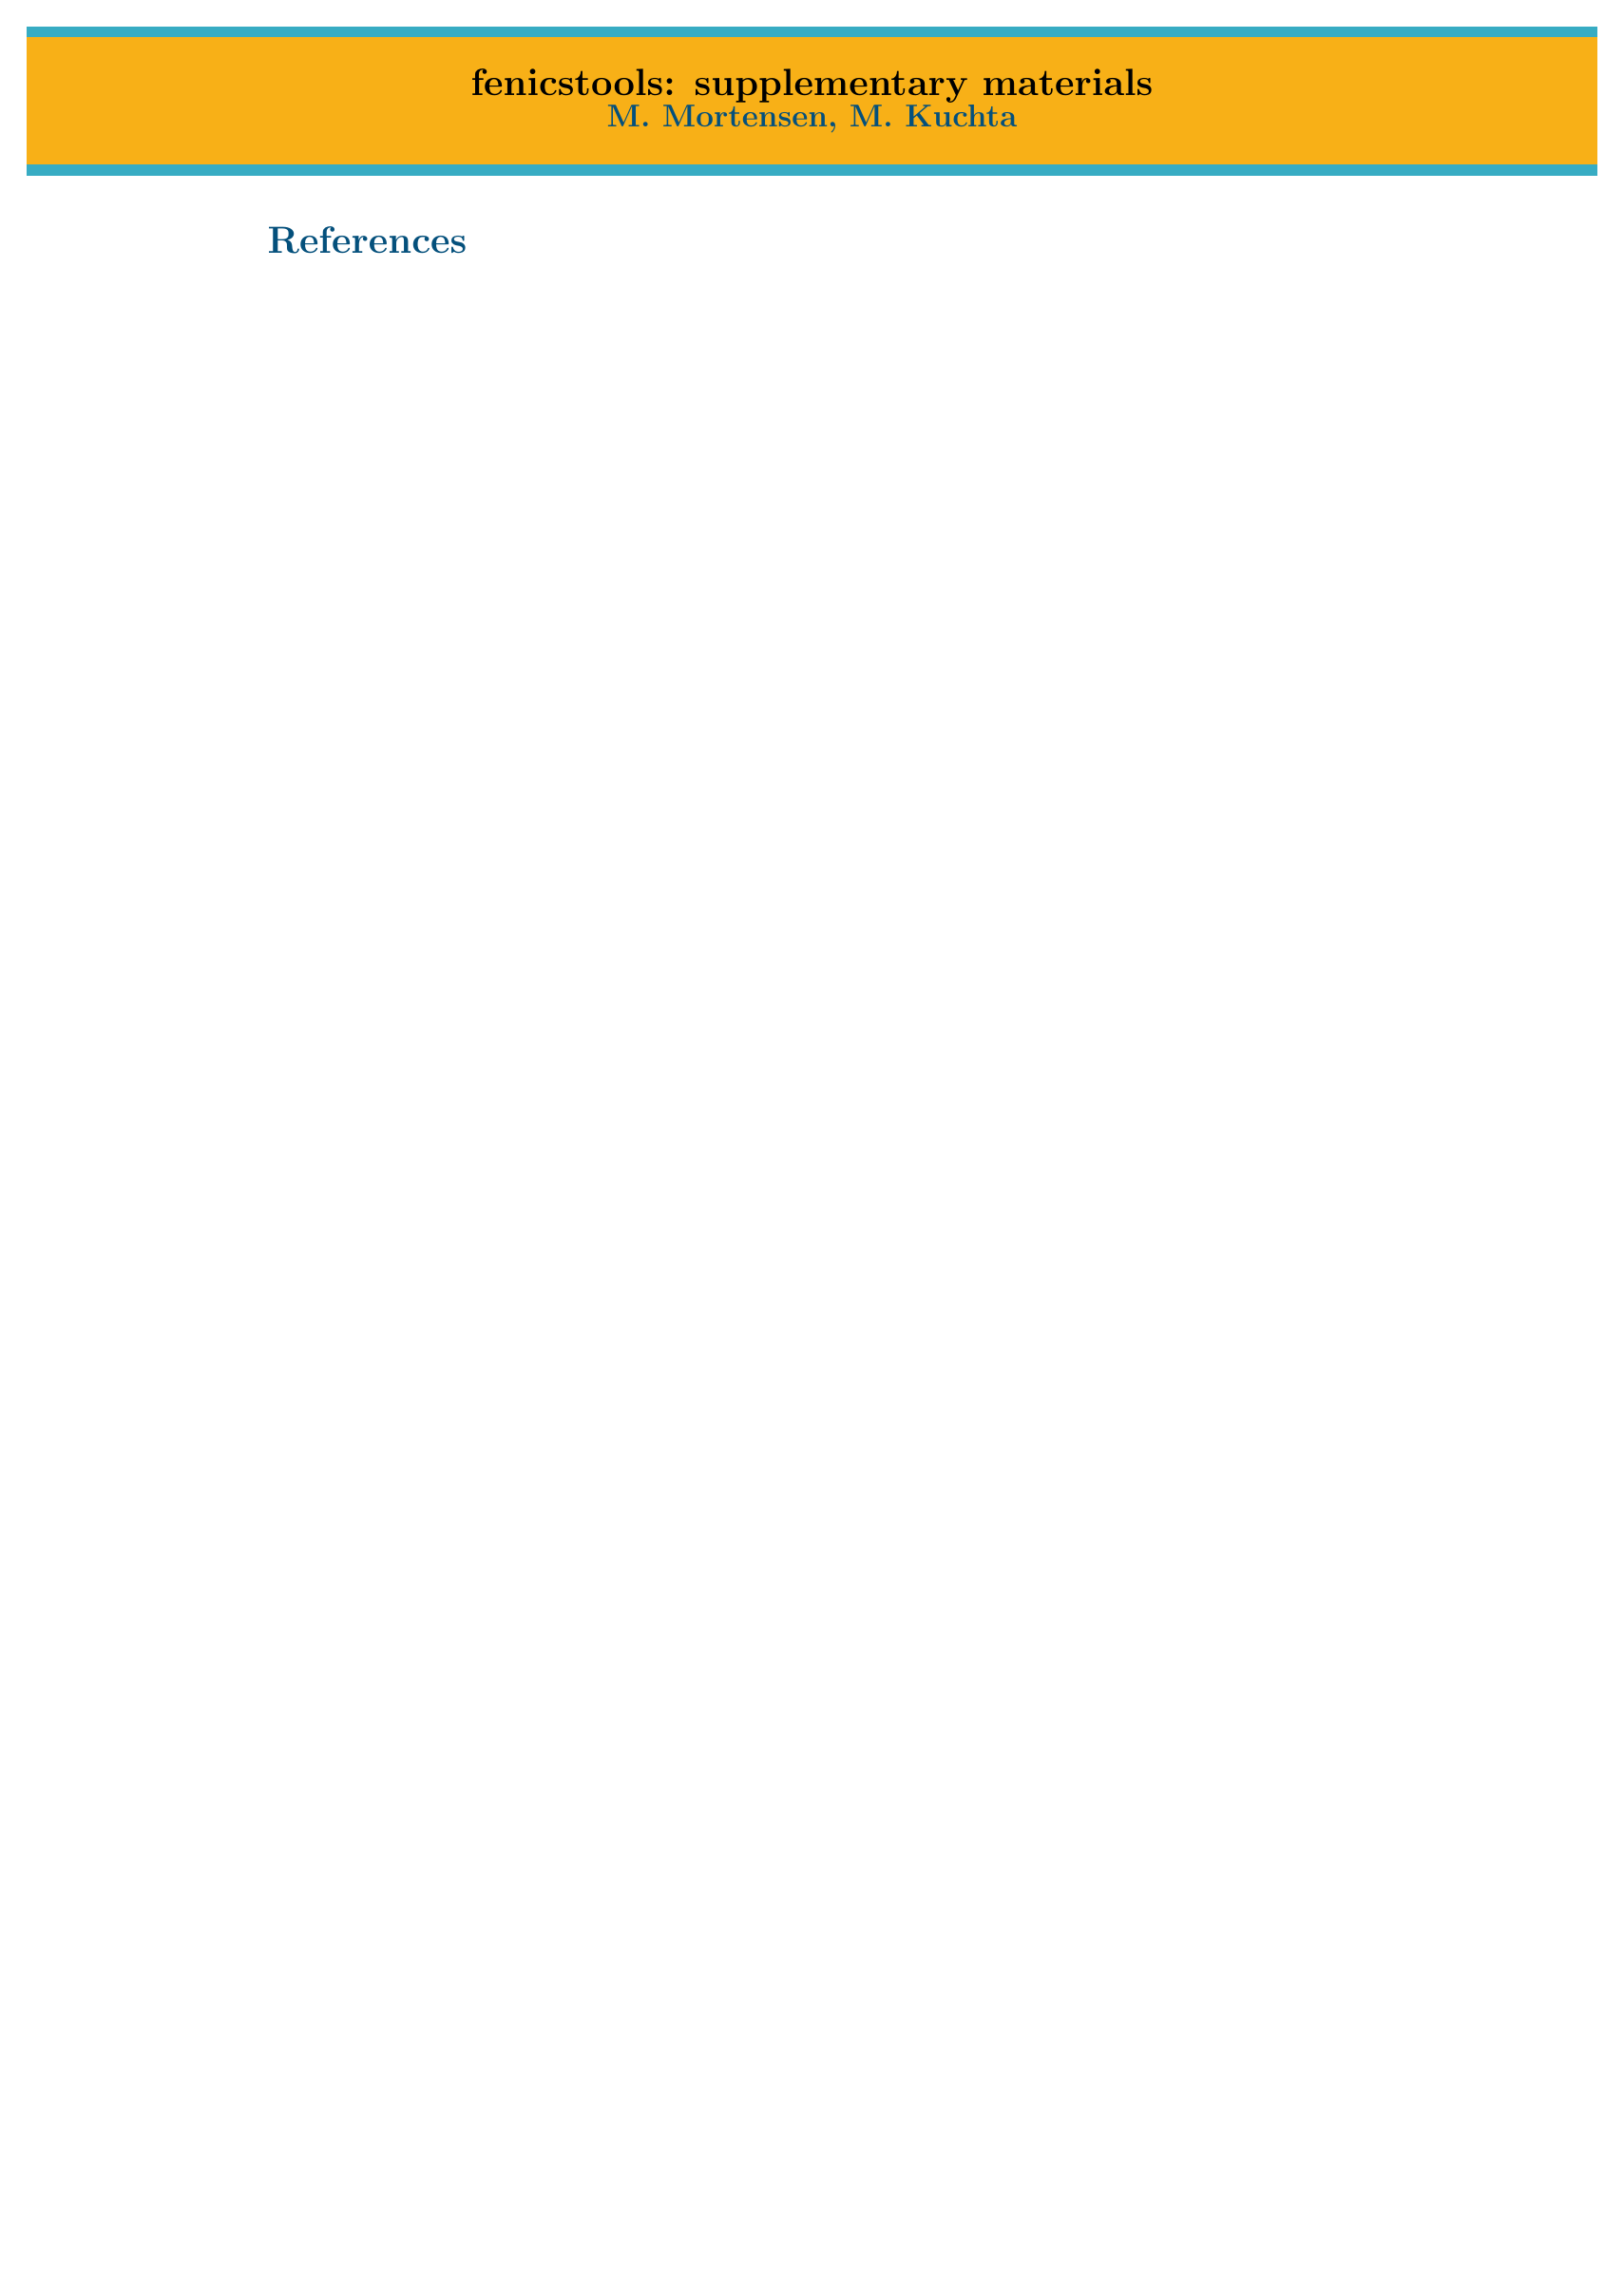
\begin{tikzpicture}[x=21cm, y=29.7cm]
\fill[white, use as bounding box] (0, 0) rectangle (1, 1);

%%%%%%%%%%%%%%%%%%%%%%%%%%
% Title
%%%%%%%%%%%%%%%%%%%%%%%%%%
\begingroup
\draw[fill=eyellow, draw=none] { 
  ($(current bounding box.north west)+(0cm, -20.0mm)$) --
  ($(current bounding box.north east)+(0cm, -20.0mm)$) -- 
  (current bounding box.north east) --
  (current bounding box.north west) -- 
  cycle
};
   %
\draw[elblue, line width=1.5mm]{
  ($(current bounding box.north east)-(0cm, 0.75mm)$) --
  ($(current bounding box.north west)-(0cm, 0.75mm)$)
};
  %
\draw[elblue, line width=1.5mm]{
  ($(current bounding box.north east)+(0cm, -19.25mm)$) --
  ($(current bounding box.north west)+(0cm, -19.25mm)$)
};
\node[anchor=center]
      (title)
      at ($(current bounding box.north)+(0cm, -1.0cm)$)
  {\begin{minipage}{\textwidth}
   \begin{center}
     {\ffmfamily\Large\bfseries\color{black}{fenicstools: supplementary materials}}\\
     {\ffmfamily\large\color{edblue}\textbf{M.~Mortensen, M.~Kuchta}}
   \end{center}
  \end{minipage}};
\endgroup


\node[anchor=north] at ($(current bounding box.north)+(0cm, -2.5cm)$)
{
  \begin{minipage}{1.2\textwidth}
    \section*{\ffmfamily\color{edblue}{References}}
    \bibliographystyle{plain}
    \vspace{-1cm}
    \bibliography{extras}
  \end{minipage}
};
\end{tikzpicture}

\end{document}
